% -----------------------------------------------------------------------------------------------------
% B3. Sources: digest.md (B3 tables), results/B3_summary.json (speed-ups, shares in orders A and B, late window,
% ratios, mu_eff_geomean, seed spread of the shares), findings.md Sec. 1. Product of the measured factors (I1--I2
% factor times mu_eff/mu) computed from the window geometric means of B3_summary.json; product of exact contractions
% versus realized V_t (seed 0) computed from results/B3.pkl with vrlab.analysis.trajectory_bounds (cut at V < 1e-18;
% ratio to V_t at the cut 5.17 and 3.41 for kappa = 1e2, 1e3, and between 0.129 and 5.52 all along, i.e. at most a
% factor 7.75; 0.955 and 0.959 after 100 passes for kappa = 1e4, 1e5; kappa = 10: V_t over the product 11 after 20
% passes, 24.1 to 1.18e3 beyond 30 passes, at most 3.07 of 19.3 decades; rho_exact(0) = 0.98616 held for n/10
% iterations gives 0.248 against V_{n/10}/V_0 = 0.691, i.e. a product of 0.359 V_t at t = n/10, 2.77-2.79 times below
% V_t on the five seeds).
% -----------------------------------------------------------------------------------------------------
\subsection{Where the proof of Proposition~5.9 loses (hypothesis B3)}\label{sec:exp-B3}

\paragraph{Question and measurements.}
Which inequalities make $\rho_{\rm bound}=1-\min\{\frac1{3n},\frac{3\mu}{16R^2}\}$ pessimistic, and how does this depend
on the conditioning and the anisotropy of the data? We run SAGA with the textbook constants ($\gamma=1/(4R^2)$,
$\Delta=3\gamma^2$) on the fifteen problems $\kappa\in\{10,\dots,10^5\}$, $\alpha\in\{0,1,2\}$, and record, with the
instruments of Section~\ref{sec:th-B3}, $\rho_{\rm exact}(t)$, the tightness ratios
$r_{\rm sq},r_{\rm coco},r_{\rm var},r_{\rm sc},r_{\rm min}$ of I1--I5 and $r_{\rm init}$ of I6, and the attribution chains of
\resref{prop:B3-attribution}, which undo the inequalities one at a time and split the logarithmic gap
$\log(1/\rho_{\rm exact})-\log(1/\rho_{\rm bound})$ into nonnegative \emph{shares}. Order~B (undo I5, I4, I2, I3, I1,
i.e.\ the intermediate rates of the proof applied cumulatively) is shown in the figures; order~A (I4, I2, I3, I1, then
I5) keeps the minimum until the end. Numbers are averages over passes 2--20 and over the 5 seeds unless stated
otherwise.

\paragraph{Size of the gap (Figure~\ref{fig:fig1}).}
The speed-up is $3.2$--$3.7$ for $\kappa\le10^2$, where the memory term $\frac1{3n}$ is the active one, and grows with
$\kappa$ in the parameter-term regime: $5.1$, $5.2$ and $3.4$ at $\kappa=10^3$, $29$, $16$ and $6.0$ at $\kappa=10^4$, $220$,
$100$ and $19$ at $\kappa=10^5$, for $\alpha=0$, $1$ and $2$ (passes 20--100: $187$, $72$ and $11$ at $\kappa=10^5$). At
$\kappa=10^4$ and $\alpha=1$, the mean squared distance decreases from $\norm{\theta_0-\etastar}^2=1954$ to $7.1\cdot10^{-9}$
in 100 passes, by $11.4$ orders of magnitude, whereas the bound only decreases by the factor $\rho_{\rm bound}^{10^5}=0.15$,
to $29\norm{\theta_0-\etastar}^2$ with the constant $1+\frac{3n}{16}$ of the proof ($38\norm{\theta_0-\etastar}^2$ with the
$1+\frac n4$ of the statement). Along seed $0$ ($\alpha=1$), the product of the exact conditional contractions agrees
with the realized $V_t$ within $5\%$ after 100 passes at $\kappa=10^4$ and $10^5$ ($11.5$ and $6.5$ decades of decrease),
and within a factor $5.2$ where the curves reach the floor at $\kappa=10^2$ and $10^3$ (about 20 decades; within a factor
$7.8$ all along). At $\kappa=10$ (not shown in Figure~\ref{fig:fig1}) the realized $V_t$, then carried by its memory
term, stalls for several passes before
dropping abruptly, and the two differ by a factor $11$ after 20 passes and by $24$ to $1.2\cdot10^3$ beyond 30 passes,
i.e.\ by up to three of 19 decades (a factor of about $2.8$ comes from holding the contraction of the fresh memory at
$t=0$ for $n/10$ iterations: the product is already $0.36\,V_t$ at $t=n/10$). The exact one-step identity thus accounts
for the observed decay, and the gap lies
essentially in the inequalities.

\begin{figure}[tbp]
  \renewcommand{\thefigure}{1}% project figure name (see the header of this file)
  \centering
  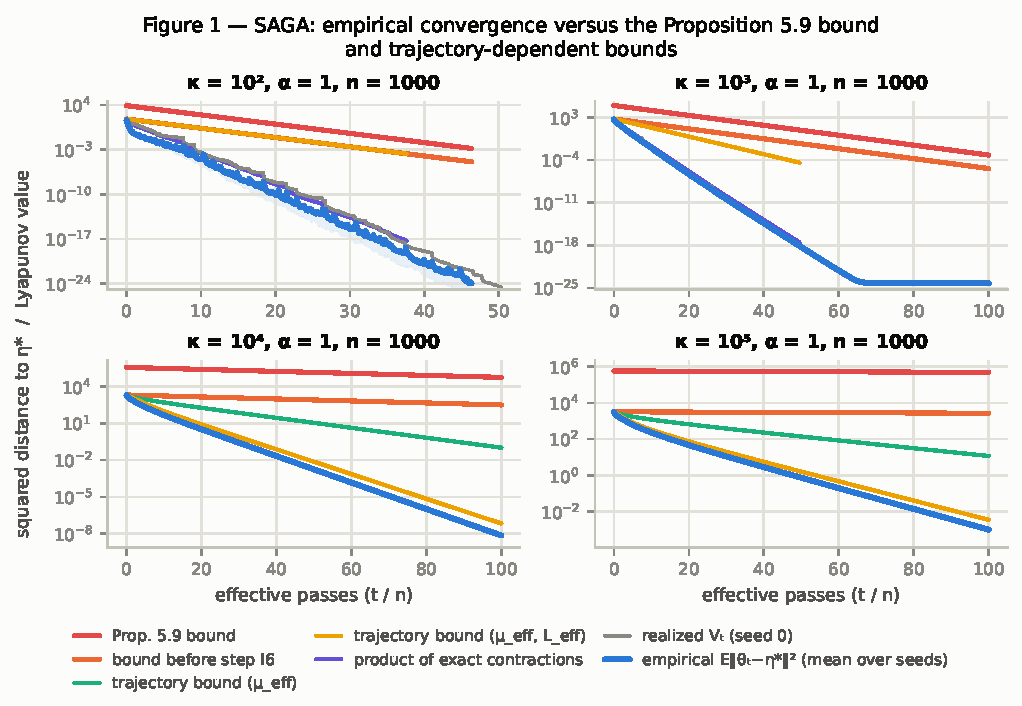
\includegraphics[width=\textwidth]{fig1_convergence_vs_bound}
  \caption{\textbf{Figure~1 of the proposal: SAGA against the bound of Proposition~\ref{prop:59}.} Logistic regression,
  $n=1{,}000$, $d=50$, $\alpha=1$, $\kappa\in\{10^2,10^3,10^4,10^5\}$ (one panel each), step $\gamma=1/(4R^2)$. Blue:
  $\E\norm{\theta_t-\etastar}^2$ estimated by the mean over 5 seeds (band: min--max); red: the bound of
  Proposition~\ref{prop:59} with the constant $1+3n/16$ obtained in its proof (the statement rounds it up to
  $1+n/4$); orange: the same bound before the initialization step I6, $\rho_{\rm bound}^tV_0$ ($V_t$ is the Lyapunov
  function of Section~\ref{sec:setting}); green and yellow: products, along the realized trajectory of seed $0$ and from its
  $V_0$, of the factors of \protect\resref{prop:B3-traj}, with $\mu$ replaced by $\muEff(\theta_{t-1})$ (green)
  and, in addition, $R^2$ replaced by $\LEff(\theta_{t-1})$ in the coefficient of the parameter term (yellow); violet:
  product of the exact conditional contractions $\rho_{\rm exact}(t)$ along the same trajectory; grey: realized Lyapunov
  value $V_t$ of seed $0$. The factors are computed every $n/10$ iterations and held constant in between. The three
  trajectory-dependent products (green, yellow, violet) are cut at the first instrumentation time with $V_t<10^{-18}$,
  below which the conditional expectations are dominated by rounding; the other curves end with the runs, which stop at
  $\norm{\theta_t-\etastar}^2\le10^{-26}$ (the mean and the two bounds with the shortest of the five). Where the memory
  term $1/(3n)$ is the active one in the a-posteriori factors ($\kappa\le10^3$ here, since $\muEff/\mu\ge16\kappa/(9n)$ along
  these runs; in the certified factor only for $\kappa\le10^2$, as $\frac3{16\kappa}<\frac1{3n}$ for $\kappa>\frac{9n}{16}$) the
  green and yellow curves coincide, and for $\kappa=10^2$ they also coincide with the orange one; for $\kappa\ge10^4$ the
  violet and grey curves are indistinguishable from the blue one and hidden under it. One legend, below the panels,
  serves all of them.}
  \label{fig:fig1}
\end{figure}

\paragraph{Tightness ratios (Figure~\ref{fig:fig2}).}
I3 and I5 are nearly tight on all fifteen problems: $r_{\rm var}\ge0.958$, because the mean stored error $\bar z$ is small
compared with the individual ones ($r_{\rm var}=1-n\norm{\bar z}^2/M$), and $r_{\rm min}\ge0.9998$. The square-norm step has
$r_{\rm sq}=0.50$--$0.52$ for $\kappa\le10^2$, the factor $2$ lost, by item~(iii) of \resref{lem:B3-ranges}, when the
gradient changes $a_i$ and the memory errors $b_i$ (the values of $a_t$ and $b_t$ of I1 when $i(t)=i$) are uncorrelated,
and $0.075$, $0.015$ and $0.0035$ at $\kappa=10^5$, where the memory is fresh relative to the slow motion of $\theta_t$, as
\resref{rem:B3-fresh} explains. Cocoercivity has $r_{\rm coco}=\LEff/R^2$ in
$[0.16,0.37]$, $[0.11,0.16]$ and $[0.019,0.18]$ for $\alpha=0,1,2$: $R^2=\max_iL_i$ overestimates the constant met along the
trajectories by a factor $2.7$ to $52$. Strong convexity has $r_{\rm sc}=\mu/\muEff$ between $0.74$ and $0.90$ at $\kappa=10$
and $0.012$, $0.027$ and $0.14$ at $\kappa=10^5$, i.e.\ $\muEff/\mu=81$, $37$ and $6.9$ against
$\lmin(F''(\etastar))/\mu=70$, $26$ and $2.1$ (the iterates are still far from $\etastar$ during passes 2--20). Finally
$r_{\rm init}$ is $3.1\cdot10^{-5}$ to $0.028$, but I6 only enters the constant $1+\frac n4$.

\begin{figure}[tbp]
  \renewcommand{\thefigure}{2}% project figure name (see the header of this file)
  \centering
  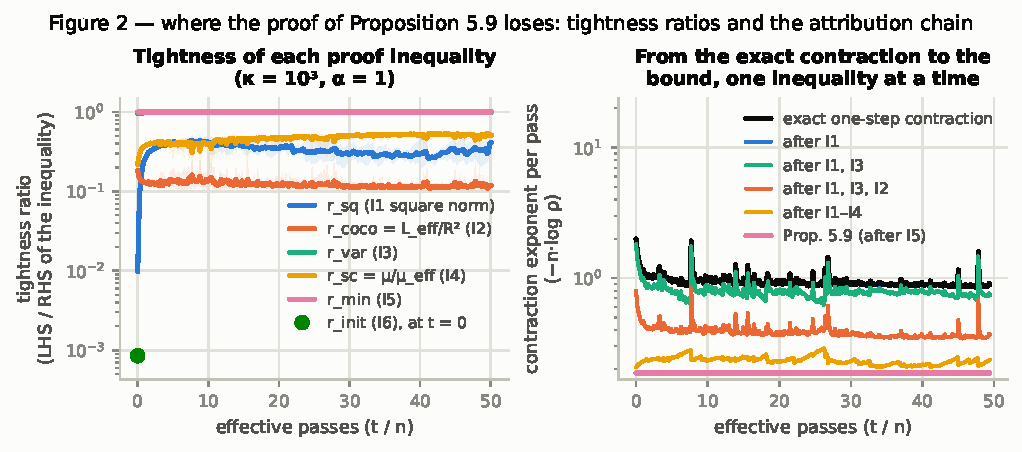
\includegraphics[width=\textwidth]{fig2_tightness_ratios}
  \caption{\textbf{Figure~2 of the proposal: tightness of each inequality of the proof.} Logistic regression,
  $n=1{,}000$, $d=50$, $\kappa=10^3$, $\alpha=1$, textbook constants. Left: tightness ratios of I1--I5
  (\protect\resref*{def:B3-ratios}: smaller side over larger side, $1$ meaning equality), computed from exact conditional
  expectations every $n/10$ iterations; geometric mean over 5 seeds (band: min--max), records with $V_t<10^{-18}$
  discarded. The ratio of the initialization inequality I6, $r_{\rm init}=8.5\cdot10^{-4}$ for this problem, is the single
  marker at $t=0$, below the other curves. Right: attribution chain along seed $0$ (order~B of
  \protect\resref*{prop:B3-attribution}, records with $V_t\ge10^{-18}$): contraction exponent per pass, $-n\log\rho$, of the
  exact one-step contraction and after applying the inequalities cumulatively in the order of the proof (I1, I3, I2,
  I4, I5), down to the certified rate of Proposition~\ref{prop:59}. The curve after I1 is hidden under the curve after
  I1 and I3, because I3 is nearly tight.}
  \label{fig:fig2}
\end{figure}

\paragraph{Attribution (Figure~\ref{fig:fig3}).}
In order~B, for $\kappa\le10^2$ the gap is carried by I1 ($0.39$--$0.44$) and I2 ($0.32$--$0.37$), then I5 ($0.07$--$0.22$)
and I4 ($0.03$--$0.17$). For $\kappa\ge10^4$, cocoercivity dominates ($0.46$ for $\alpha=0$, $0.54$--$0.58$ for $\alpha=1$,
$0.62$--$0.71$ for $\alpha=2$), strong convexity follows ($0.25$--$0.36$), and together they carry $0.77$--$0.96$ of the
gap, while I1 falls to $0.03$--$0.16$ and I5 to at most $0.073$; at $\kappa=10^3$ and $\alpha=2$, I2 alone carries $0.83$.
Over the grid the largest share of I3 is $0.54\%$ and that of I5 is $22\%$ (a ratio as close to $1$ as $r_{\rm min}$
still matters because the exponents are small: at $\kappa=10$, I5 adds about $2\cdot10^{-4}$ per iteration to a certified
exponent of $3.3\cdot10^{-4}$); the seed-to-seed spread of the shares is below $0.03$ for $\kappa\ge10^4$. Order~A also
gives I3 a small share (at most $0.006$, except $0.063$ at $\kappa=10^3$, $\alpha=2$) and gives $0.59$--$0.96$ to I4 and I2 together
for $\kappa\ge10^4$, but for $\kappa\le10^2$ it gives $0.56$--$0.61$ to the minimum I5, $0.38$--$0.44$ to I1 and nothing to
I4 and I2, which only lower the parameter coefficient, not the active one there: as \resref{rem:B3-orders} explains, the
attribution is order dependent where the two components of $V_t$ compete.

\begin{figure}[tbp]
  \renewcommand{\thefigure}{3}% project figure name (see the header of this file)
  \centering
  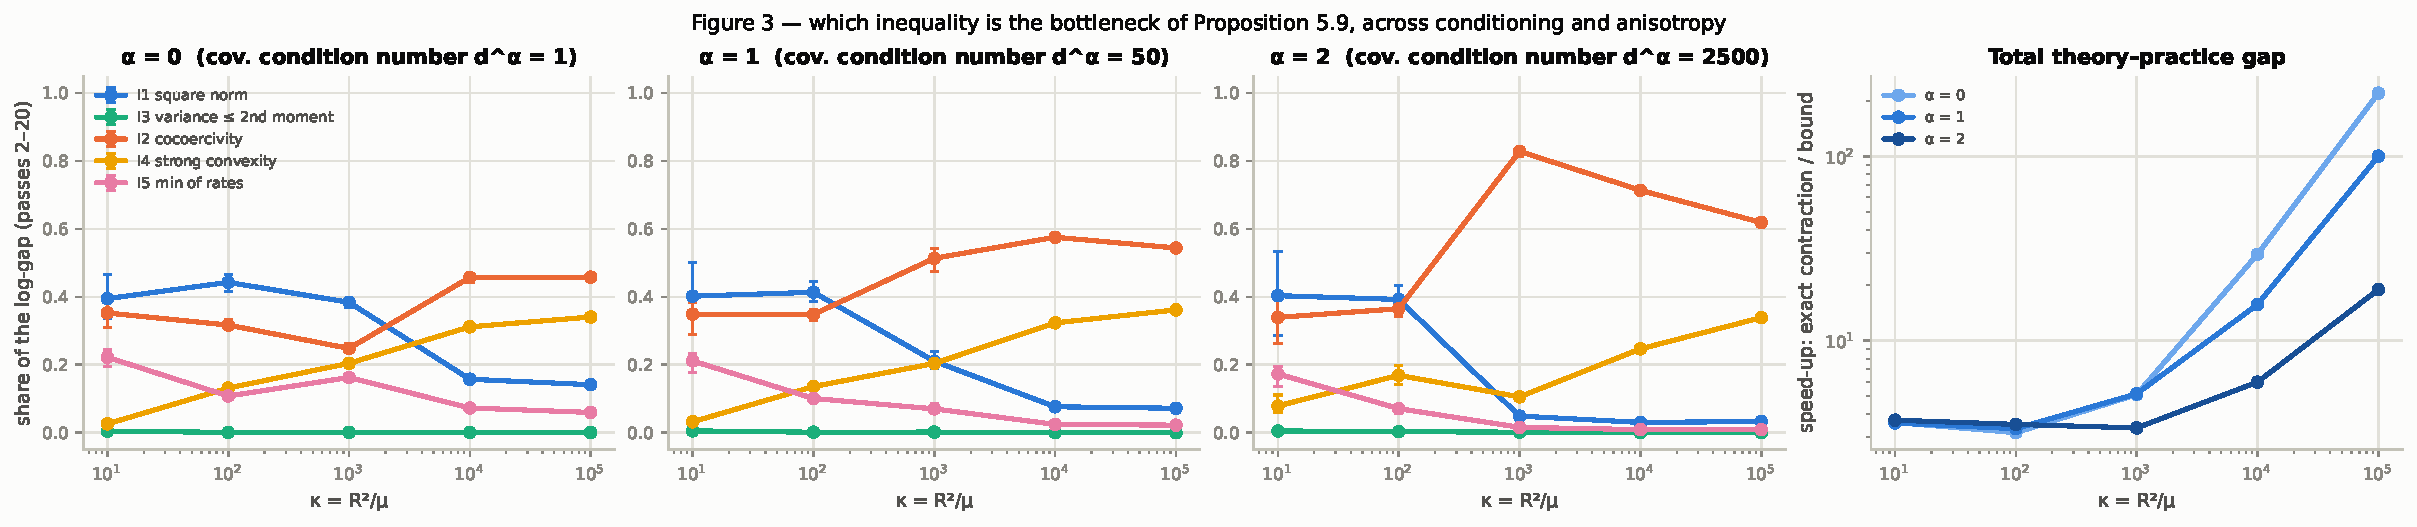
\includegraphics[width=\textwidth]{fig3_bottleneck_by_geometry}
  \caption{\textbf{Figure~3 of the proposal: which inequality is the bottleneck.} Share of the logarithmic gap between the
  exact one-step contraction and the certified one attributed to each inequality (order~B of
  \protect\resref*{prop:B3-attribution}, i.e.\ cumulative attribution in proof order), averaged over passes 2--20
  (records with $V_t\ge10^{-18}$) and over 5 seeds (error bars: min--max over seeds), as a function of $\kappa$, for the
  covariance spectra $j^{-\alpha}$, $\alpha\in\{0,1,2\}$ (top left, top right and bottom left; population condition numbers
  $1$, $50$, $2500$); logistic regression, $n=1{,}000$, $d=50$, textbook constants. Bottom right: total speed-up factor
  $(-\log\rho_{\rm exact})/(-\log\rho_{\rm bound})$ (window average, mean over seeds).}
  \label{fig:fig3}
\end{figure}

\paragraph{Interpretation.}
By \resref{prop:B3-representation} the exact parameter coefficient is
$1-\frac{\muEff}{2R^2}\big(1-r_{\rm coco}(\frac{r_{\rm sq}}4+\frac38)\big)$: relative to the worst case, I4 multiplies the
parameter exponent by $\muEff/\mu\in[1,\kappa]$ (item~(i) of \resref*{lem:B3-ranges}), and I1 and I2 together by
$\big(1-r_{\rm coco}(\frac{r_{\rm sq}}4+\frac38)\big)/\frac38\in[1,\frac83]$ at the fixed step
(\resref*{rem:B3-fixed-step}). For $\kappa\ge10^4$, where the parameter term is active and $D_t$ carries most of $V_t$
($r_{\rm min}\approx1$), inserting the window geometric means of the ratios into this product reproduces $0.91$--$0.96$ of
the measured speed-ups: $\muEff/\mu$ (between $2.2$ and $81$) times a factor $2.45$--$2.62$ from I1 and I2. The
$\kappa$-dependent part of the gap is thus the strong-convexity step, the difference between $\mu=\lambda$ and the
curvature met along the trajectory; cocoercivity contributes a bounded factor, whose larger additive share in order~B
comes from acting on an exponent already multiplied by $\muEff/\mu$. With strongly anisotropic features ($\alpha=2$) the
bottom of the spectrum of $F''(\etastar)$ stays close to $\lambda$, so I4 is closer to tight and I2 dominates the shares.
The large factors at $\kappa=10^5$ are a property of these instances, not of the order of the bound: by
\resref{prop:B3-lower} no analysis of SAGA with a constant step can improve the exponent $1$ of $\kappa$
uniformly over the class of Proposition~\ref{prop:59} (caveat~(ii) of \resref*{rem:B3-conclusion}).

% -----------------------------------------------------------------------------------------------------
% Constants. Sources: results/GammaDelta_summary.json, digest.md "(gamma, Delta) inside the proof", per-seed rates
% in results/GammaDelta.pkl (all three seeds converge at every step); B3 note Prop. B3-optimum, Cor. B3-c.
% kappa <= 1e2 (findings.md Sec. 4; B3 note, paragraph "Comparison with the textbook choice", Remark rem:B3-conclusion
% and Outcome): at gamma = 1/(4R^2) the best c is c_Delta = (6s-16+sqrt((6s-16)^2+128s))/(2s), s = n/kappa, = 5.036 and
% 5.894, with rate (6-c)/(16 kappa) = 1.8085 and 1.9821 times 1/(3n); Q(10) = 2.4223, Q(100) = 2.9400; speed-ups of
% B3_summary.json divided by these: 1.754--1.945 and 1.217--1.452; c_exact_per_iter / (-log(1-1/n)) = 1.057--1.236.
% -----------------------------------------------------------------------------------------------------
\subsection{The constants of the proof}\label{sec:exp-constants}

Is the gap a matter of the convenient constants $\gamma=1/(4R^2)$ and $\Delta=3\gamma^2$? \resref{prop:B3-optimum} gives
the best pair $(\gamma,\Delta)$ in closed form; by \resref{rem:B3-conclusion}, it improves the certified rate by a factor
between $1.05$ and $3$, and by at most $\frac43$ when $\kappa\ge9n/16$. At $\kappa=10^3$ the
optimum is $\gamma R^2=0.219$, $\Delta=2.56\gamma^2$, with certified rate $2.19\cdot10^{-4}$ per iteration against
$1.875\cdot10^{-4}$, a gain of $17\%$. On logistic regression ($\kappa=10^3$, $\alpha=1$, 3 seeds, slopes over passes 2--40,
Figure~\ref{fig:C}) the observed exponent per pass is $0.51$, $0.97$, $1.14$, $1.09$, $0.95$, $0.66$ and $0.027$ for
$\gamma R^2=\frac18$, $\frac14$, $\frac13$, $\frac12$, $1$, $2$ and $4$, whereas the best certificate is $0.18$, $0.22$ and $0.17$
for the first three steps and does not exist for $\gamma R^2\ge\frac12$, where, by \resref{cor:B3-c}, no $\Delta$ is
admissible. At the textbook step the observed exponent is $4.5$ times the best certificate, and SAGA,
fastest around $\gamma R^2=\frac13$, still converges for all three seeds at $\gamma R^2=4$, eight times the supremum
$\frac12$ of the steps $\gamma R^2$ that the proof admits. The constants of Proposition~\ref{prop:59} are thus within $17\%$
of the best ones of their proof at this conditioning, and the factor $4.5$ left at the textbook step is the slack of the
inequalities (\resref*{rem:B3-conclusion}); the admissible range $\gamma R^2<\frac12$ itself comes from absorbing the
second moment $\gamma^2\Omega_{t-1}$ of the step and the memory refresh with the worst-case bounds I1--I3.

These conclusions concern $\kappa=10^3\ge\frac{9n}{16}$, where the textbook rate is the parameter term and the constants
can gain at most $\frac43$. For $\kappa\le10^2$, where it is the memory term $\frac1{3n}$, the constants account for a
larger part of the speed-ups $3.2$--$3.7$ of Section~\ref{sec:exp-B3}: at the textbook step, the best weight,
$\Delta=c\gamma^2$ with $c\approx5.04$ ($\kappa=10^2$) or $c\approx5.89$ ($\kappa=10$) instead of $c=3$, multiplies the
certified rate by $1.81$ or $1.98$, and the optimal constants of \resref*{prop:B3-optimum}, at a smaller step, by $2.42$
or $2.94$, leaving factors $1.75$--$1.95$ and $1.22$--$1.45$, respectively. The exact exponents $-\log\rho_{\rm exact}$
there (passes 2--20, mean over the seeds) are $1.06$--$1.24$ times $-\log(1-\frac1n)$, the largest exponent $-\log\rho$
of a bound $\E[V_t]\le c_0\rho^tV_0$ with $c_0$ independent of $t$, whatever $\Delta$ (\resref*{rem:B3-conclusion}): a
typical trajectory of $V_t$ decreases faster than its expectation can.

\begin{figure}[tbp]
  \renewcommand{\thefigure}{C}% project figure name (see the header of this file)
  \centering
  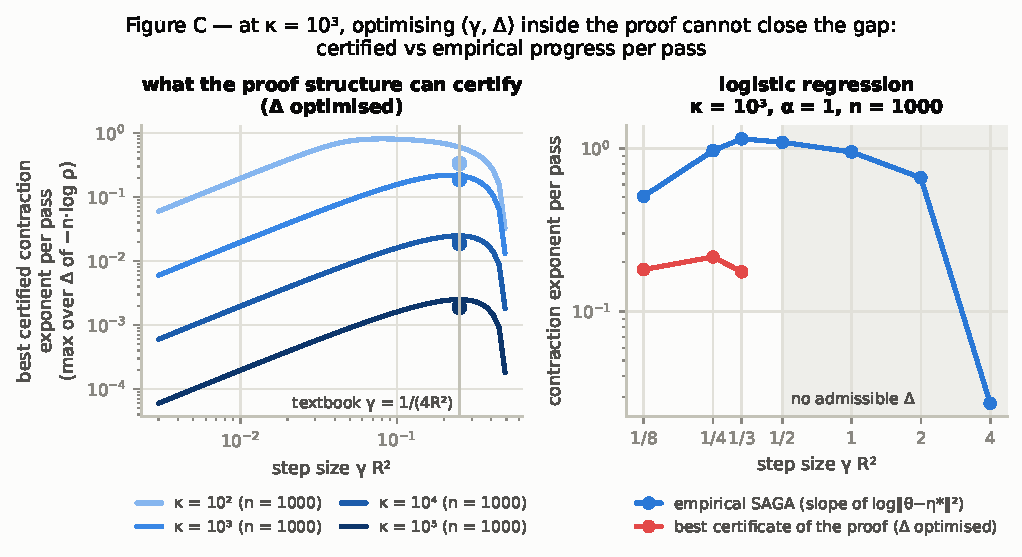
\includegraphics[width=\textwidth]{figC_gamma_delta}
  \caption{\textbf{The constants inside the proof.} Left: best contraction exponent per pass that the proof structure of
  Proposition~\ref{prop:59} can certify, as a function of the step $\gamma R^2$, with the Lyapunov weight $\Delta=c\gamma^2$
  optimized over $c$ (\protect\resref*{cor:B3-c}), for $\kappa\in\{10^2,10^3,10^4,10^5\}$ and $n=1{,}000$; dots: textbook
  constants $\gamma=1/(4R^2)$, $\Delta=3\gamma^2$. Right: logistic regression ($\kappa=10^3$, $\alpha=1$, $n=1{,}000$, $d=50$),
  empirical contraction exponent per pass of SAGA (least-squares slope of $\log\norm{\theta_t-\etastar}^2$ over passes
  2--40, mean over 3 seeds) and best certificate of the proof at the same step; the proof certifies nothing for
  $\gamma R^2\ge\frac12$, where no $\Delta$ is admissible (shaded region).}
  \label{fig:C}
\end{figure}
